% ---------------------------------------------------------------------------
% Savant: structure-free protein-ligand affinity prediction for ligand
% screening on CPU.
%
% Figures are produced by report/make_figures.py into report/figures/.
% ---------------------------------------------------------------------------
\documentclass[times, twoside]{zHenriquesLab-StyleBioRxiv}

\usepackage{graphicx}
\usepackage{multirow}
\usepackage{booktabs}
\usepackage{amsmath}
\usepackage{xcolor}
% \usepackage{hyperref}

\graphicspath{{figures/}}

%% Custom Commands
\usepackage{xspace}
\newcommand{\savant}{\textit{Savant}\xspace}
\newcommand{\pl}{protein--ligand\xspace}
\newcommand{\Pl}{Protein--ligand\xspace}
\newcommand{\pkd}{\ensuremath{\mathrm{pK_d}}\xspace}

\leadauthor{Guirales-Medrano}

\begin{document}

\title{Savant: Fast, Structure-Free Protein-Ligand Affinity Prediction Enabled Ligand Screening}
\shorttitle{Savant: Structure-Free Protein-Ligand Affinity Prediction}

\author[1,2,\Letter]{Sayal Guirales-Medrano}
\author[1,2,3]{Colby T. Ford}
\author[1,2]{Daniel Janies}

\affil[1]{Center for Computational Intelligence to Predict Health and Environmental Risks (CIPHER), University of North Carolina at Charlotte, USA}
\affil[2]{Department of Bioinformatics and Genomics, University of North Carolina at Charlotte, USA}
\affil[3]{Tuple LLC, Charlotte, NC USA}

\maketitle

\begin{abstract}
\Pl binding affinity is the central quantitative measurement of early drug discovery, because it determines which of many candidate molecules is worth synthesizing and assaying. Bringing a single medicine to market now requires a median capitalized investment near \$1 billion, while generative chemistry and make-on-demand catalogs produce candidate molecules faster than any rigorous method can evaluate them. Leading computational methods close this gap by co-folding the \pl complex before scoring it, which is accurate but requires a graphics processing unit (GPU) and substantial time for every pair evaluated.

We developed \savant, a model that predicts the dissociation constant of a \pl pair from an amino acid sequence and a Simplified Molecular-Input Line-Entry System (SMILES) string alone, with no experimental structure, no predicted structure, no docking, and no GPU. We built the model in 2 stages. We first trained a structure-based model on 47,619 complexes folded with AlphaFold3 and refined with HADDOCK3, and we measured how its accuracy scales with the number of complexes produced. The docked energy terms were worth 0.051 in the coefficient of determination, and the learning curve rose by 0.058 per doubling of training data with no sign of saturation. Because folding the remaining 97.4\% of the corpus was not feasible, we removed the structure and acquired accuracy from data instead, training on 1.8 million measured pairs using protein and ligand language-model embeddings, physicochemical descriptors, and a topological fingerprint.

To evaluate the model, we assembled a benchmark of 500 \pl pairs across 20 targets, restricted to measurements published in 2025 or later and to ligands below an Extended Connectivity Fingerprint Tanimoto similarity of 0.50 to anything in training. We report accuracy separately for the 2 abilities that a pooled correlation blends. \savant achieved the highest within-target correlation of any method tested ($r = 0.436$, compared to 0.386 for Boltz-2), and the highest mean within-target rank correlation across the 20 targets ($\rho = 0.278$, compared to 0.228 for Boltz-2). Conversely, \savant does not rank targets against one another, and no method tested, including \savant, predicted absolute affinity more accurately than predicting the benchmark mean. We show that this last result follows from the label: replicate measurements of the same pair disagree by 0.81 \pkd, which caps the achievable coefficient of determination on this benchmark at approximately 0.60 and drives predictions toward the mean. The marginal cost of scoring 1 additional ligand against an already-encoded target is 0.018 s on a central processing unit, which projects to approximately half an hour for a library of 100,000 compounds. We conclude that removing the structure trades away absolute calibration and retains the ability that ligand screening actually requires, which is ranking many molecules against 1 protein.
\end{abstract}

\begin{center}
    \begin{keywords}
    Binding Affinity | Protein-Ligand Interactions | Drug Discovery \\Virtual Screening | Machine Learning | Protein Language Models
    \end{keywords}

    \begin{corrauthor}
    sguirale@charlotte.edu
    \end{corrauthor}
\end{center}

% ===========================================================================
\section*{Introduction}
% ===========================================================================

Bringing a new medicine to market is among the most expensive undertakings in applied science. Wouters et al. estimated the median capitalized research and development investment per approved medicine at \$985.3 million, with a mean of \$1,335.9 million, across 63 drugs approved between 2009 and 2018~\cite{wouters2020cost}. Industry-sourced estimates are higher still, reaching \$2,558 million capitalized per approval~\cite{dimasi2016innovation}. Scannell et al. documented that the number of new drugs approved per billion dollars of research and development spending has halved roughly every 9 years since 1950, an approximately 80-fold decline in inflation-adjusted terms~\cite{scannell2012eroom}. Computational inputs have become dramatically cheaper over the same period while output has not improved, which places a premium on methods that triage candidates early and inexpensively~\cite{paul2010improve}.

That premium has grown sharply because the supply of candidate molecules has outrun our ability to evaluate them. Lyu et al. docked 170 million make-on-demand compounds against 2 targets~\cite{lyu2019ultralarge}, VirtualFlow extended open-source screening past 1 billion compounds~\cite{gorgulla2020virtualflow}, and ZINC-22 now catalogs tangible compounds at multi-billion scale~\cite{tingle2023zinc22}. Generative models add to this supply directly, producing novel structures under property constraints~\cite{olivecrona2017reinvent,blaschke2020reinvent2}. This results in a practical problem: $10^9$ to $10^{10}$ of available molecules but rigorous per-compound takes a long time to process. Sadybekov and Katritch state that fast, cost-effective screening is the step that would let these libraries be used at the scale at which they are being created~\cite{sadybekov2023computational}.

Binding affinity is the quantity that would resolve the triage problem if it could be predicted cheaply. Affinity is commonly expressed through the dissociation constant ($K_d$), which relates to the free energy of binding through $\Delta G = -RT \ln K_d$~\cite{gilson2007calculation}. \Pl binding is governed by an interplay of hydrogen bonding, electrostatic interactions, hydrophobic effects, van der Waals interactions, and desolvation~\cite{gilson2007calculation}, and the practical limits of optimizing it against molecular size motivated ligand efficiency as a design metric~\cite{hopkins2004ligand}. Experimental determination by surface plasmon resonance, isothermal titration calorimetry, or fluorescence-based assays remains the gold standard against which all computational work is calibrated, but these assays require purified material and operate far below the throughput at which candidate molecules are now produced.

Physics-based computational methods span a wide accuracy and cost range, and neither end of that range solves the triage problem. At the inexpensive end, docking programs place ligands well but score them poorly: in a critical assessment of 10 docking programs and 37 scoring functions across 8 targets, no program or scoring function produced useful rank-order predictions of compound affinity~\cite{warren2006critical}, and the CASF-2016 comparative assessment shows that even best-case scoring correlations remain modest~\cite{su2019casf2016}. At the expensive end, alchemical free-energy methods do achieve predictive accuracy, tested across 8 targets and 199 ligands~\cite{wang2015fep} and comparable performance in prospective industrial projects~\cite{schindler2020largescale}. Free-energy perturbation, however, requires a high-quality structure, a congeneric ligand series, and GPU-hours per compound, which together rule it out for library-scale triage.

Advances in structure prediction appeared to remove the first of those requirements. AlphaFold3 predicts biomolecular complexes including \pl systems~\cite{abramson2024alphafold3}, and open co-folding models now predict structure and affinity together~\cite{wohlwend2024boltz1,passaro2025boltz2,corso2023diffdock}. The evidence that this transfers to affinity is weaker than it first appears. Karelina et al. found that although AlphaFold2 models capture binding-pocket structure well, ligand poses predicted from those models were not significantly more accurate than poses from traditional homology models, and were substantially less accurate than poses predicted from experimentally determined structures~\cite{karelina2023alphafold}. A predicted structure is therefore not yet a substitute for a measured one when the downstream task is quantitative.

A parallel line of work predicts affinity without any structure at all. DeepDTA established that \pkd can be predicted from sequence and SMILES alone~\cite{ozturk2018deepdta}, and subsequent methods refined the representation using molecular graphs~\cite{nguyen2021graphdta}, interaction transformers~\cite{huang2021moltrans}, contrastive protein-language embeddings~\cite{singh2023conplex}, and bilinear attention with domain adaptation~\cite{bai2023drugban}. PLAPT is the closest published peer to the present work, combining protein and chemical language-model embeddings in a small neural head~\cite{rose2024plapt}. The featurizers themselves have improved independently: protein language models now recover structural information from sequence alone~\cite{lin2023esm2,esmc2024}, and chemical language models pretrained on tens of millions of SMILES provide transferable molecular representations~\cite{chithrananda2020chemberta,ahmad2022chemberta2}. Standardized collections support comparison across these methods~\cite{huang2021tdc}.

How such methods are evaluated is itself contested, and this is central to the argument we make here. Chen et al. showed that apparent deep-learning enrichment on DUD-E derived from analogue and decoy bias in the dataset rather than from learning \pl interactions~\cite{chen2019dude}. Wallach and Heifets demonstrated that most ligand-based classification benchmarks reward memorization rather than generalization~\cite{wallach2018memorization}, and Sieg et al. formalized the bias controls needed to avoid this~\cite{sieg2019bias}. Volkov et al. reached the harshest conclusion for affinity regression specifically, finding that an explicit description of \pl noncovalent interactions provided no advantage over ligand-only or protein-only descriptors, and that memorization largely dominated true learning~\cite{volkov2022frustration}; related analyses of graph networks reach compatible conclusions about what such embeddings encode~\cite{mastropietro2023gnn}. A single correlation pooled over many targets is vulnerable to exactly this failure, because a model can score well by recognizing which target a pair belongs to. We therefore separate the pooled correlation into a between-target component and a within-target component and report them individually. We present this decomposition as our operationalization of the warnings above for the affinity-regression setting.

Any claim about predictive accuracy must also be read against the precision of the measurements being predicted. Kramer et al. quantified the experimental uncertainty of heterogeneous public $K_i$ data at a mean error of 0.44 and a standard deviation of 0.54 $\mathrm{p}K_i$, and argued that this uncertainty defines a natural upper limit on achievable predictive performance, such that models reporting smaller errors are necessarily overtrained~\cite{kramer2012uncertainty}.

Here we present \savant, a gradient-boosted model that predicts \pkd from sequence and SMILES alone. We chose gradient-boosted trees because the feature set is heterogeneous tabular data combining embeddings, descriptors, and fingerprints, a regime in which tree ensembles remain competitive with deep networks and are robust to uninformative features~\cite{chen2016xgboost,grinsztajn2022tabular,shwartzziv2022tabular}. We report how we arrived at the design as well as the design itself. We first built a structure-based model, measured what the docked structure contributed, and measured how that contribution scaled. We then used those measurements to justify removing the structure. Finally, we trained the structure-free model toward the screening objective directly and evaluated it on a temporally separated, ligand-novel benchmark against methods that require a GPU and methods that require a structure. Our aim throughout was a model that runs on hardware any laboratory already owns, which is the condition under which fast screening becomes broadly accessible~\cite{sadybekov2023computational}.

% ===========================================================================
\section*{Methods}
% ===========================================================================

\subsection*{Data acquisition and preparation}

We sourced \pl data from the public Hugging Face dataset \href{https://huggingface.co/datasets/jglaser/binding_affinity}{jglaser/binding\_affinity}, compiled by Jens Glaser~\cite{glaser_binding_affinity}. The dataset aggregates records from BindingDB~\cite{gilson2016bindingdb}, PDBbind-CN~\cite{wang2004pdbbind,liu2015pdbbind}, BioLiP~\cite{yang2013biolip}, and Binding MOAD~\cite{hu2005bindingmoad}. It comprises 1.8 million pairs of protein amino acid sequences (\texttt{seq}) and ligand SMILES strings (\texttt{smiles}) with a measured affinity, provided both in micromolar units (\texttt{affinity\_uM}) and as a negative logarithm in molar units (\texttt{neg\_log10\_affinity\_M}).

We used \pkd in molar units as the prediction target throughout, defined in Equation~\ref{eq:pktokd}.

\begin{equation}
\pkd = -\log_{10}\!\left(K_d\;[\mu\mathrm{M}]\right) + 6
\label{eq:pktokd}
\end{equation}

Two properties of this label govern the interpretation of every result reported below, and both are properties of the measurement rather than of any model.

First, the label pools assay types. The released file provides a single affinity column and no \texttt{standard\_type} field, so dissociation constants ($K_d$), inhibition constants ($K_i$), and half-maximal inhibitory concentrations (IC$_{50}$) are mixed and cannot be separated after the fact.

Second, the label is noisy, and we quantified the noise directly. We found that 11.9\% of unique sequence and SMILES pairs appear more than once in the corpus, and that these replicates disagree by a pooled standard deviation of 0.81 \pkd. A model that recovered the true value exactly would therefore still record a root mean squared error (RMSE) of approximately 0.81 against single measurements. This exceeds the approximately 0.5 $\mathrm{p}K_i$ uncertainty that Kramer et al. reported for filtered public data~\cite{kramer2012uncertainty}. We read every error figure in this study against that floor, not against zero.

We collapsed replicate measurements of the same pair to their median before fitting, so that a frequently re-measured pair does not receive proportionally more weight than a singly measured one. We discarded pairs whose replicates disagreed by more than 1.5 \pkd as irreconcilable. We also identified measurements recorded at the standard censoring concentrations of 10, 100, 1,000, and 10,000 $\mu$M, which are reporting limits and not true measurements, and we excluded them from the regression target while retaining them as negatives for classification.

\subsection*{Structural biology workflow}

We sampled 50,000 records and processed them through an AI-based folding and interaction quantification workflow. This workflow uses AlphaFold3~\cite{abramson2024alphafold3} to fold the amino acid sequence into a protein structure, construct the small molecule, and place the ligand within the protein.

We then evaluated each docked complex using HADDOCK3~\cite{haddock3} with a \texttt{[topoaa]} topology generation stage followed by an \texttt{[emref]} energy minimization stage. From the resulting Critical Assessment of PRedicted Interactions (CAPRI) table we read 6 energy terms: \texttt{score}, \texttt{total}, \texttt{vdw}, \texttt{elec}, \texttt{desolv}, and \texttt{bsa}. These map onto the thermodynamic decomposition of binding described by Gilson and Zhou~\cite{gilson2007calculation}. We computed a seventh geometric term directly from the pose, defined as the count of protein residues having any atom within 6.0 \AA{} of any ligand atom.

We used RDKit~\cite{rdkit} to derive additional features of the complex, including molecular weight, LogP, the number of hydrogen bond donors and acceptors, the number of rotatable bonds, topological polar surface area, the number of rings, the number of aromatic rings, the number of atoms, the number of heavy atoms, and formal charge.

Of the 50,000 sampled complexes, 47,619 completed successfully. This constituted the structure-based training set.

\subsection*{Isolating the contribution of the docked structure}

To measure what the docked structure was worth, we trained 2 models that differ in exactly 1 respect. Both consume a ChemBERTa-77M-MLM~\cite{ahmad2022chemberta2} ligand embedding (384 dimensions), an ESM2-8M~\cite{lin2023esm2} protein embedding (320 dimensions), RDKit descriptors computed on the hydrogen-added molecule (11 columns) together with the surviving RDKit descriptor set (212 columns, after dropping columns constant across the training data), an Extended Connectivity Fingerprint of diameter 4 (ECFP4) count fingerprint~\cite{rogers2010ecfp} (1,024 dimensions), and amino acid composition with chain length (21 columns). We mean-pooled all embeddings over the last hidden state with padding masked out. The structure-based model additionally receives the 7 HADDOCK3 terms, giving 1,979 features against 1,972. The difference between the 2 therefore isolates the contribution of the docked structure.

We fitted both variants with XGBoost~\cite{chen2016xgboost} under 3 held-out regimes: protein-grouped, in which no protein is shared between training and test; ligand-grouped; and both-disjoint. Rows from different regimes are not comparable to one another, because each regime defines its own test set. The comparison that carries meaning is structure-based against structure-free within a single regime.

\subsection*{Learning-curve experiment}

The structure-based model used 47,619 docked complexes, which is 2.6\% of the available pairs. Producing the remainder would require compute we did not have. To determine whether that compute would be worthwhile, we measured the shape of the learning curve directly.

We fixed a single protein-grouped test set at the outset and did not modify it thereafter. We then trained models on increasing fractions of the remaining pairs (0.1, 0.2, 0.3, 0.4, 0.6, 0.8, and 1.0), with and without the HADDOCK3 block at every size, and we repeated each size over independent subsamples so that we could report the spread across repeats alongside the mean. Because the test set is fixed, points on the curve are comparable to one another, which would not be the case if each size drew its own split.

\subsection*{Structure-free model}

Folding 1.8 million complexes was not feasible within this project. We therefore removed the structure entirely and acquired accuracy from data instead. We retained every feature derivable from the sequence and the SMILES string and trained on the full corpus.

We encoded the protein with ESM2-650M~\cite{lin2023esm2}, which produces a 1,280-dimensional representation, and the ligand with ChemBERTa-77M-MLM~\cite{ahmad2022chemberta2}, which produces 384 dimensions. We mean-pooled both over the last hidden state with padding masked out. To these we added the surviving RDKit named descriptor set, an ECFP4 count fingerprint~\cite{rogers2010ecfp}, and amino acid composition with chain length. Table~\ref{tab:blocks} gives the resulting layout.

\begin{table}[h]
\centering
\caption{Feature layout of the reported model. Block order is load-bearing and must match the order used in training.}
\label{tab:blocks}
\small
\begin{tabular}{llr}
\toprule
Block & Source & Width \\
\midrule
ChemBERTa-77M-MLM ligand embedding  & SMILES   & 384 \\
RDKit named descriptors             & SMILES   & 226 \\
ECFP4 count fingerprint             & SMILES   & 1,024 \\
ESM2-650M protein embedding         & sequence & 1,280 \\
Amino acid composition and length   & sequence & 21 \\
\midrule
\multicolumn{2}{l}{Total}                      & 2,935 \\
\bottomrule
\end{tabular}
\end{table}

\subsection*{Model training}

We fitted the model with XGBoost~\cite{chen2016xgboost} under squared-error loss and a protein-grouped split, in which no protein is shared between the training and test sets. The inner split used for early stopping holds out the same grouping key as the outer split. A random inner split would allow the model to tune against proteins on which it is subsequently tested, which inflates the reported score without improving the model.

We averaged replicate measurements of the same sequence and SMILES pair into a single label before fitting, so that a frequently re-measured pair does not receive proportionally more weight than a singly measured one. We also removed benchmark ligands from the training set before fitting, dropping every training ligand within an ECFP4 Tanimoto similarity of 0.50 of any benchmark ligand, so that the benchmark cannot measure memorization.

The model ships as a regressor alone. We make binder calls by thresholding the predicted \pkd, which has the additional advantage that the threshold is selected at inference time and is not fixed during training.

Table~\ref{tab:training} reports the held-out performance the model reached during training. This test set is a protein-grouped hold-out drawn from the training corpus, so it measures generalization to unseen proteins within the same data distribution. It is not the external benchmark, and the 2 should not be compared directly.

\begin{table}[h]
% source: ML_model/models_full/variant_comparison.csv, row esm650
\centering
\caption{Held-out performance of the reported model during training, on a protein-grouped test split of the training corpus.}
\label{tab:training}
\small
\begin{tabular}{lr}
\toprule
Quantity & Value \\
\midrule
Features                          & 2,935 \\
Fitting pairs                     & 1,022,678 \\
Validation pairs                  & 229,846 \\
Held-out test pairs               & 315,792 \\
Boosting rounds at best iteration & 1,784 \\
\midrule
Test $R^2$                        & 0.307 \\
Test Pearson $r$                  & 0.564 \\
Test Spearman $\rho$              & 0.536 \\
Test RMSE                         & 1.270 \\
Test MAE                          & 1.026 \\
Constant-baseline RMSE            & 1.526 \\
Predicted / true spread           & 0.508 \\
\bottomrule
\end{tabular}
\end{table}

On this split the model explains 30.7\% of the variance in \pkd and beats the constant baseline on RMSE, at 1.270 against 1.526. Both figures are stronger than the corresponding ones on the external benchmark reported below, which is the expected consequence of a hold-out drawn from the same distribution and the same period as the training data.

\subsection*{Benchmark construction}

To evaluate the model we assembled a benchmark of 500 \pl pairs across 20 targets from ChEMBL~\cite{gaulton2012chembl,zdrazil2024chembl}. We constructed the set to be difficult in 3 specific respects.

\begin{itemize}
  \item Ligand novelty. Every benchmark ligand falls below an ECFP4 Tanimoto similarity of 0.50 to anything in \savant's training set. The realized maximum is 0.494.
  \item Temporal separation. Every measurement dates from 2025 or later and is absent from ChEMBL v34 (April 2024), the release most plausibly contained within the training window of the comparison methods.
  \item Assay filtering. We retained $K_d$ and $K_i$ measurements only, at a ChEMBL confidence score of 8 or greater.
\end{itemize}

This design is a time split in the sense of Sheridan, who showed that random cross-validation is optimistic and that splitting on measurement date estimates prospective performance far more realistically~\cite{sheridan2013timesplit}. Combined with the near-neighbor removal, it implements directly what the memorization literature recommends for benchmarks intended to measure generalization~\cite{wallach2018memorization,sieg2019bias}.

We deliberately did not require novel proteins. The training corpus covers essentially every well-measured target, so a novel-protein requirement would have left only sparsely characterized targets, for which the ground truth is itself unreliable. All 20 benchmark targets therefore appear in training with other ligands. This benchmark measures the ranking of novel chemistry against an established target, which is the realistic screening scenario, and results obtained from it must not be described as zero-shot with respect to the target.

The temporal filter protects every method equally, because no method trained before 2025 can have seen these measurements. The ligand similarity filter does not transfer between methods, and the direction in which this cuts is worth stating explicitly. We applied the near-neighbor removal to \savant's training set only. The comparison methods were trained by other groups on other corpora and may retain close analogues of these benchmark ligands. \savant is therefore held to a stricter novelty standard than the methods against which we compare it, and any advantage it shows is measured under that handicap.

We audited the training corpus against the benchmark before every reported run, computing for each benchmark ligand its maximum ECFP4 Tanimoto similarity to the training set, whether its InChIKey skeleton appears in training, and whether the exact pair appears in training. We report a result only when all 3 checks return zero violations.

\subsection*{Comparison methods}

Table~\ref{tab:tools} lists the methods compared and the input each requires at inference time.

\begin{table}[h]
\centering
\caption{The methods compared, and the input each requires at inference time.}
\label{tab:tools}
\small
\begin{tabular}{p{0.16\columnwidth}p{0.48\columnwidth}p{0.22\columnwidth}}
\toprule
Method & Description & Requires \\
\midrule
\textbf{\savant} & This work. Gradient-boosted trees over protein and ligand language-model embeddings, physicochemical descriptors, and a topological fingerprint & sequence and SMILES, CPU \\
\textbf{Boltz-2} & Co-folds the \pl complex with a diffusion model, then predicts affinity from the predicted structure & sequence and SMILES, GPU \\
\textbf{PRODIGY-LIG} & Physics-based rescoring. A linear model over atomic contact counts in an existing complex & a 3-dimensional complex \\
\textbf{PLAPT} & The closest published peer. Protein and chemical language-model embeddings passed to a small neural head, also structure-free & sequence and SMILES \\
\bottomrule
\end{tabular}
\end{table}

Boltz-2 represents the co-folding approach and is the strongest generally available affinity predictor we could run~\cite{passaro2025boltz2}. PRODIGY-LIG represents physics-based rescoring and requires a structure, which we supplied from the same folding workflow used in the structure-based stage~\cite{vangone2019prodigylig}. PLAPT is the closest structure-free peer~\cite{rose2024plapt} and is, at the time of writing, a preprint that has not undergone independent peer review.

\subsection*{Evaluation and statistical analysis}

We decomposed the pooled Pearson correlation into a between-target component, which correlates predicted target means against measured target means, and a within-target component, which centers both quantities on the target mean beforehand. The first corresponds to determining which protein binds more tightly and the second to determining which ligand binds more tightly for a given target. This decomposition is not a standard named analysis in this field; we introduce it here as a quantitative operationalization of the qualitative warnings that pooled benchmarks reward exploiting target identity~\cite{chen2019dude,wallach2018memorization,sieg2019bias,volkov2022frustration}.

We computed Spearman $\rho$ within every target carrying at least 10 pairs and averaged across targets. We deliberately do not report enrichment factors. Truchon and Bayly showed that the enrichment factor is insensitive to ranking performance before and after its cutoff~\cite{truchon2007bedroc}, and our benchmark is 88.6\% binders, a density at which enrichment saturates near 1.13 and cannot separate a perfect ranker from a mediocre one.

We computed all paired comparisons as cluster-resampled bootstraps, resampling targets instead of individual pairs, so that the resulting interval reflects uncertainty over the units actually sampled. We report Wilcoxon signed-rank and sign tests alongside each bootstrap. All confidence intervals are 95\%, and we report a point estimate whose interval spans zero as parity, irrespective of the sign of the estimate. For paired comparisons of within-target correlations we additionally applied the test of Steiger~\cite{steiger1980}, which accounts for the dependence between 2 correlations measured against the same values and is therefore more sensitive than comparing 2 independent intervals.

\subsection*{Runtime measurement}

We measured runtime on CPU, with the protein encoder forced onto CPU explicitly, because the presence of a visible GPU otherwise alters the measurement even when the GPU is not intended to be used. We measured 3 quantities separately, because they scale differently: the one-off cost of encoding a protein, the marginal cost of 1 additional ligand scored against an already-encoded protein, and the total for a realistic mixed workload. We did not take a head-to-head wall-clock measurement of Boltz-2. The runtime comparison reported below is therefore structural, describing the work each method must perform per pair, and is not a measured speedup ratio.

% ===========================================================================
\section*{Results}
% ===========================================================================

\subsection*{Docked structural terms improve prediction across all splits}

Table~\ref{tab:phase1} shows the held-out performance of the structure-based and structure-free models on the docked subset.

\begin{table}[h]
% source: ML_model/models_structure_free/results.csv
\centering
\caption{Held-out performance on the 47,619 docked complexes. Rows are not comparable across splits, because each split defines its own test set.}
\label{tab:phase1}
\small
\begin{tabular}{llrrrr}
\toprule
Features & Split & $n$ test & $R^2$ & $r$ & RMSE \\
\midrule
structure-free  & protein & 9,116  & 0.400 & 0.633 & 1.163 \\
structure-free  & ligand  & 10,998 & 0.440 & 0.667 & 1.123 \\
structure-free  & both    & 2,291  & 0.355 & 0.599 & 1.261 \\
structure-based & protein & 9,116  & 0.451 & 0.673 & 1.112 \\
structure-based & ligand  & 10,998 & 0.491 & 0.704 & 1.071 \\
structure-based & both    & 2,291  & 0.385 & 0.623 & 1.232 \\
\bottomrule
\end{tabular}
\end{table}

Under the protein-grouped split, the docked model reached $R^2 = 0.451$, compared to $R^2 = 0.400$ for the identical model with the HADDOCK3 block removed. We observed this advantage consistently across all 3 splits. The docking terms were worth approximately 0.05 in $R^2$ and 0.035 in $r$. The docked structure therefore contributes real information. However, the question that follows is not whether it helps but whether it is the most efficient way to spend compute.

\subsection*{Performance continues to rise with additional docked complexes}

To determine whether producing additional docked complexes would improve the model further, we measured the learning curve. In Fig.~\ref{fig:curve} we see the result.

\begin{figure}[h]
\centering
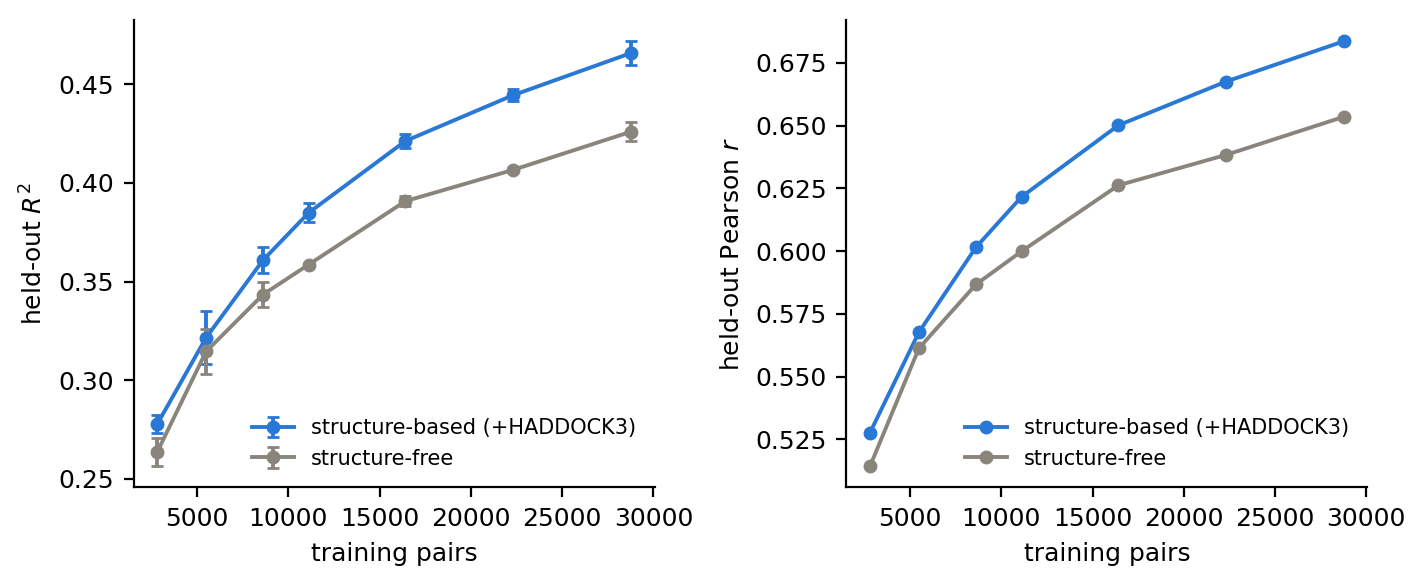
\includegraphics[width=\columnwidth]{fig_learning_curve.png}
\caption{Learning curve computed on a fixed protein-grouped test set, with and without the HADDOCK3 block at every training size. The left panel shows the coefficient of determination and the right panel shows the Pearson correlation. Error bars show the spread across repeated subsamples of the same size. Data source: \texttt{learning\_curve\_summary.csv}.}
\label{fig:curve}
\end{figure}

Two quantities emerge from this experiment. First, the curve has not flattened. Over the final segment, the docked model moved from $R^2 = 0.445$ at 22,302 pairs to $R^2 = 0.466$ at 28,767 pairs, which corresponds to a slope of 0.058 in $R^2$ per doubling of the training data. We observed no sign of saturation at the largest size reached. Notably, this result indicates that folding additional complexes would continue to improve the model, and the slope provides an approximate budget for how much compute purchases how much accuracy.

Second, the structural contribution is modest and does not vary with scale. Averaged over all training sizes, the HADDOCK3 block is worth 0.025 in $R^2$, and in Fig.~\ref{fig:curve} we see that the gap between the 2 series neither closes nor widens materially as the training set grows.

Both readings extrapolate beyond the measured range, and their magnitude should not be quoted at 1.8 million pairs. What the curve establishes is the direction and the approximate rate, not the value at the full corpus.

\subsection*{The learning curve motivates removing the structure}

These 2 measurements together determine the design of the model. A gain of 0.025 in $R^2$ that costs minutes of folding and refinement per complex compares unfavorably against a gain of 0.058 in $R^2$ per doubling that costs only additional rows, particularly when approximately 40 times more rows were already available and undocked. Folding the remaining 1.85 million complexes was not achievable with the GPU allocation and time available to this project, and the learning curve indicates that the same accuracy is more cheaply purchased with data that already exists.

We therefore removed the structure. We emphasize that this is a resource argument rather than a claim that structure is uninformative. The docked terms helped in every split we measured, and a project with sufficient GPU capacity to fold the full corpus would be expected to do better than the model reported here.

\subsection*{No method predicts absolute affinity better than a constant}

The evaluation set holds 500 pairs across 20 targets and 373 distinct ligand skeletons, with a mean \pkd of 7.296 and a standard deviation of 1.274. The realized maximum ECFP4 Tanimoto to anything in training is 0.494. That label spread of 1.274 \pkd is the value against which every RMSE below should be judged, because it is precisely the RMSE achieved by predicting the benchmark mean for every pair. Table~\ref{tab:benchmark} reports every method against it.

\begin{table}[h]
% source: bench_A_pooled.csv, bench_A_decomposition.csv, bench_B_summary.csv
\centering
\caption{The 4 compared methods on the 500-pair benchmark. Between-target $r$ corresponds to determining which protein binds more tightly and within-target $r$ to determining which ligand binds more tightly for a given target. Mean $\rho$ is the within-target Spearman correlation averaged over the 20 targets. Boltz-2 and PRODIGY-LIG returned no prediction for 4 pairs.}
\label{tab:benchmark}
\small
\begin{tabular}{lrrrrrr}
\toprule
Method & $n$ & Between $r$ & Within $r$ & Pooled $r$ & Mean $\rho$ & RMSE \\
\midrule
\savant           & 500 & 0.100 & \textbf{0.436} & 0.227 & \textbf{0.278} & 1.353 \\
Boltz-2           & 496 & \textbf{0.351} & 0.386 & \textbf{0.412} & 0.228 & 1.388 \\
PRODIGY-LIG       & 496 & 0.295 & 0.237 & 0.333 & 0.233 & 1.537 \\
PLAPT             & 500 & $-0.225$ & 0.208 & 0.021 & 0.067 & 1.827 \\
\midrule
Constant baseline & 500 & ---   & ---   & ---   & ---   & \textbf{1.273} \\
\bottomrule
\end{tabular}
\end{table}

Two findings follow from this table, and both concern the benchmark itself more than any individual method.

First, no method outperformed the constant baseline on RMSE. \savant's RMSE of 1.353 is the lowest of any method tested and is lower than Boltz-2's 1.388, but it remains higher than the 1.273 obtained by predicting 7.296 for every pair. We therefore report no absolute-error claim for any method evaluated on this benchmark, including our own.

This outcome is what the label precision predicts, following the argument of Kramer et al. that experimental uncertainty sets an upper limit on achievable performance~\cite{kramer2012uncertainty}. Treating the replicate disagreement of 0.81 \pkd as the noise standard deviation and the benchmark label spread of 1.274 \pkd as the total, the implied signal variance is $1.274^2 - 0.81^2 = 0.97$, so the reliability ratio is $0.97/1.62 = 0.60$. A model that recovered the true affinity perfectly would therefore reach an $R^2$ of approximately 0.60 and an RMSE of approximately 0.81 on this benchmark, not 1.0 and 0. The negative $R^2$ values we observe reflect a benchmark whose dynamic range is narrow relative to its measurement noise, and they are not by themselves evidence that a method is uninformative.

Second, \savant's pooled correlation of 0.227 trails both Boltz-2 (0.412) and PRODIGY-LIG (0.333). \savant also produces the most compressed predictions of any method tested, at 0.425 of the measured spread. This compression is a consequence of fitting squared-error loss against a label whose own replicate disagreement is 0.81 \pkd, which makes a prediction near the conditional mean the loss-minimizing choice. Because rank order is invariant to a change of scale, the compression does not affect any of the ranking metrics reported below; it does mean that compounds should be selected by rank, such as the top 1\% of a library, and not by an absolute predicted cutoff.

\subsection*{Decomposition reveals that \savant's accuracy is within-target}

To identify the source of \savant's pooled deficit, we decomposed the pooled correlation into its between-target and within-target components. In Fig.~\ref{fig:benchmark} we see the result alongside the calibration figures.

\begin{figure}[h]
\centering
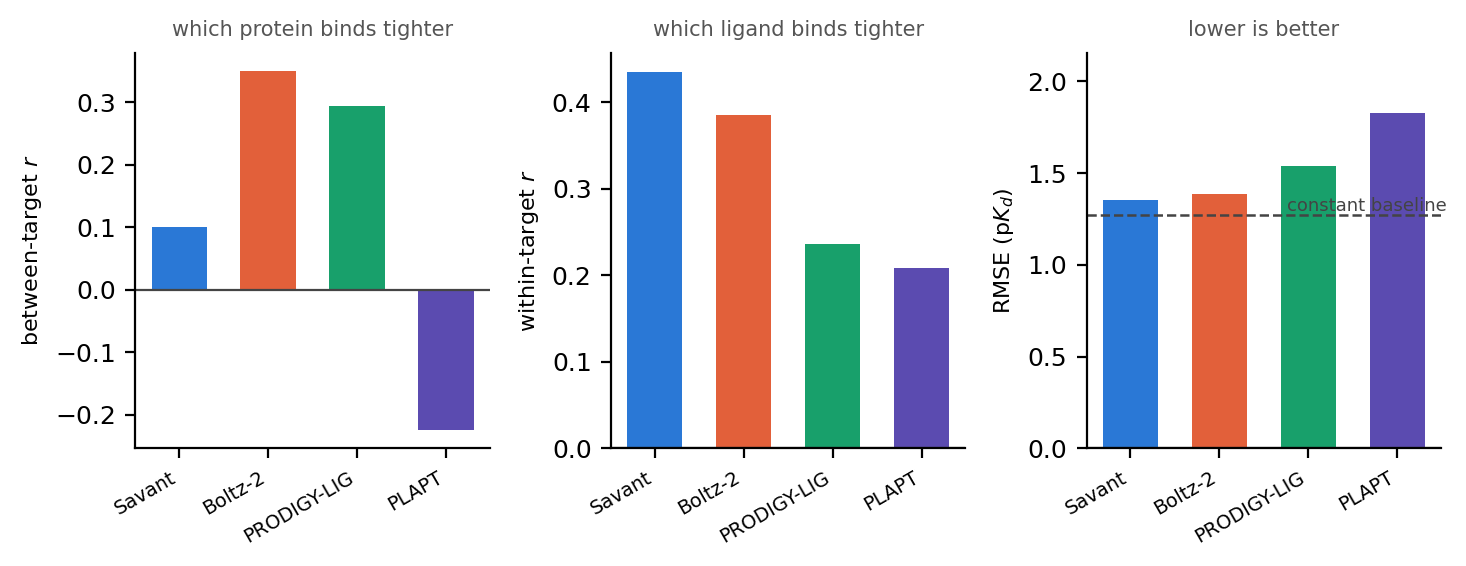
\includegraphics[width=\columnwidth]{fig_benchmark.png}
\caption{The 4 compared methods on the 3 quantities that matter. \savant achieves the highest within-target correlation and nearly the lowest between-target correlation, whereas Boltz-2 is balanced across the 2. The pooled correlation in Table~\ref{tab:benchmark} is a weighted blend of the first 2 panels, and the weighting is a property of the benchmark. In the third panel every method sits above the constant baseline. Data sources: \texttt{bench\_A\_decomposition.csv} and \texttt{bench\_A\_pooled.csv}.}
\label{fig:benchmark}
\end{figure}

This is the central result of the evaluation. \savant's within-target correlation of 0.436 is the highest of any method tested and exceeds Boltz-2's 0.386. Conversely, \savant's between-target correlation of 0.100 is close to zero and far below Boltz-2's 0.351. The pooled deficit is therefore attributable entirely to the between-target component, and on the within-target component \savant leads. These findings indicate that \savant ranks compounds against a given target at least as well as a method that folds every complex on a GPU, and that it does not reliably determine which of 2 proteins binds more tightly.

We tested these differences with Steiger's paired test on the rows for which both methods returned a prediction. \savant's advantage over PRODIGY-LIG ($P = 0.0002$) and over PLAPT ($P < 0.0001$) is larger than sampling noise. Its 0.046 advantage over Boltz-2 is not ($P = 0.24$), which is the basis on which we describe the 2 methods as at parity on this axis.

We note that the between-target axis of this benchmark is adversarial by construction. Because we selected pairs to span affinity bins within each target, the per-target mean affinity of the benchmark correlates at $r = -0.17$ with the per-target median of the training corpus. A model is therefore penalized on this axis for correctly learning a target's average level. This property explains part, though not all, of the between-target deficit, and it is a reason to prefer the decomposed figures over the pooled one.

\subsection*{\savant ranks compounds within a target as well as Boltz-2}

To evaluate the screening task directly, we computed Spearman $\rho$ within each of the 20 benchmark targets and averaged across them, which is the Mean $\rho$ column of Table~\ref{tab:benchmark}. \savant recorded the highest value of any method tested, at 0.278 against Boltz-2's 0.228, and a positive correlation on 16 of 20 targets against Boltz-2's 15.

A cluster bootstrap over targets puts the paired difference against Boltz-2 at $+0.050$, with a 95\% confidence interval from $-0.059$ to 0.159. The interval spans zero, so we report this as parity: with 20 targets the resolution available does not separate 0.278 from 0.228. The same comparison against PRODIGY-LIG gives $+0.005$ ($-0.144$ to 0.176) and against PLAPT $-0.161$ ($-0.305$ to $-0.019$). What the comparison establishes is that a model requiring no structure and no GPU is not measurably worse at the screening task than a model that folds every complex.

\subsection*{The cost of screening is dominated by encoding the protein once}

Table~\ref{tab:runtime} reports measured CPU timings.

\begin{table}[h]
% source: bench_runtime.csv
\centering
\caption{Measured CPU timings, with the protein encoder forced onto CPU.}
\label{tab:runtime}
\small
\begin{tabular}{lr}
\toprule
Quantity & CPU \\
\midrule
Protein encoding, per protein (one-off)            & 1.691 s \\
Per additional ligand against an encoded protein   & 0.018 s \\
Cold single pair, end to end                       & 1.710 s \\
500 pairs across 20 targets (the full benchmark)   & 42.9 s \\
1 target against 100,000 ligands (projected)       & 0.505 h \\
\bottomrule
\end{tabular}
\end{table}

The result here is the cost structure, not the absolute timing. The expensive step is encoding the protein, and it is performed once per target. Each additional ligand costs 0.018 s, because the marginal path consists of descriptor computation and tree inference, neither of which benefits substantially from a GPU. Screening 1 target against 100,000 compounds is therefore projected at approximately half an hour on a CPU.

This constitutes a structural advantage over co-folding methods rather than a constant-factor one. A method that folds the complex must repeat its expensive step for every ligand, so its cost is linear in library size with a large constant, whereas \savant's cost is linear with a small constant plus a fixed offset. We did not take a head-to-head wall-clock measurement against Boltz-2, and we therefore quote no speedup ratio.

% ===========================================================================
\section*{Discussion}
% ===========================================================================

In this study we built a \pl affinity predictor in 2 stages, measured what the docked structure contributed at each stage, and used those measurements to justify moving forward without structures. We then evaluated the resulting structure-free model on a temporally separated, ligand-novel benchmark against a co-folding method, a physics-based rescoring function, and the closest structure-free peer. Our central finding is that the ability to predict affinity decomposes into 2 separable abilities that are not equally difficult, and that a method can lead decisively on 1 while trailing on the other.

\subsection*{The metric selects the winner}

The ordering of methods by pooled correlation is close to the inverse of the ordering by within-target correlation. Boltz-2 leads on the pooled figure at 0.412 against \savant's 0.227, and \savant leads on the within-target figure at 0.436 against Boltz-2's 0.386. Both numbers are computed on the same 500 pairs. The difference is entirely attributable to how each metric weights the between-target and within-target components, and that weighting is a property of the benchmark rather than of any method.

That the choice of metric can reorder methods is not itself new. Truchon and Bayly made the argument for virtual-screening classification, showing that the enrichment factor and the area under the ROC curve rank methods differently because they weight early recognition differently~\cite{truchon2007bedroc}. The bias literature makes the complementary point that pooled benchmarks can be satisfied by exploiting dataset structure rather than by learning interactions~\cite{chen2019dude,wallach2018memorization,sieg2019bias}, and Volkov et al. showed for affinity regression specifically that explicit interaction descriptions add nothing over ligand-only descriptors, with memorization dominating true learning~\cite{volkov2022frustration}. What we add is a quantitative decomposition for the regression setting, and a demonstration that on a contamination-controlled benchmark the inversion is large enough to reverse the ranking of a GPU co-folding method and a CPU tree ensemble.

We therefore argue that reporting a single pooled correlation for a \pl affinity method is insufficient, because the pooled figure blends an ability that screening requires with an ability that screening never exercises. A screening campaign fixes the protein. Under that condition the between-target component is not merely less important, it is unobservable, and a method's score on it carries no information about how it will perform.

\subsection*{Why removing the structure was the correct trade under our constraints}

The learning curve is the load-bearing measurement of this paper, because it converts an intuition into a budget. The docked HADDOCK3 terms provided a 0.025 increase in $R^2$ averaged across training sizes, and that value did not grow with scale. Additional training rows were worth 0.058 in $R^2$ per doubling, and that curve had not begun to flatten at the largest size we reached. With approximately 40 times more rows already available and undocked, and with folding costing minutes per complex on a limited resource of GPUs, the math favors data over structure. This is consistent with the broader observation that predictive power in this domain scales with data volume~\cite{ramsundar2015multitask}.

Two independent lines of published evidence support the same conclusion. Volkov et al. found that explicitly describing \pl noncovalent interactions gave no advantage over ligand or protein descriptors alone~\cite{volkov2022frustration}, which is a strong external statement that the marginal value of structural detail is small. Karelina et al. found that predicted protein structures do not yet support ligand-pose prediction at the accuracy that experimentally determined structures do~\cite{karelina2023alphafold}, which means that the structures available at scale are not the structures the method would want. Our measured 0.051 in $R^2$ from the docked block sits comfortably within what those results would lead one to expect.

\subsection*{Ranking is the quantity a screening decision consumes}

A screening decision consumes an ordering. When a chemist selects the top 1\% of a library for synthesis, that choice is unchanged by any monotone transformation of the predicted values, so what matters is how closely the predicted order matches the measured one. $R^2$ and RMSE answer a different question, namely how much of the variance in the measured values a method reproduces on the original scale, and the distinction between ranking quality and calibration is well established in virtual-screening evaluation~\cite{truchon2007bedroc}.

That distinction is what reconciles \savant's leading within-target correlation with the RMSE figures in Table~\ref{tab:benchmark}. Measurement noise caps the achievable $R^2$ on this benchmark near 0.60 for any method whatsoever, and every method we tested fell below the constant baseline on RMSE, so the calibration figures characterize the benchmark and its label at least as much as they characterize the models. The ranking figures are the ones a campaign acts on, and on those \savant leads: a within-target correlation of 0.436 against Boltz-2's 0.386, and a positive rank correlation on 16 of the 20 benchmark targets.

\subsection*{Where the method applies}

\savant is built for the case in which the protein is fixed and many candidate ligands must be ordered, which covers hit triage, library prioritization, and the iterative rounds of early lead optimization. This is the common situation in practice, because a project commits to a target long before it commits to a chemical series, and most decisions that follow concern which molecules to make next.

The cost structure has the same shape as the task. Encoding the protein costs 1.691 s and happens once per target, after which each additional ligand costs 0.018 s, so a library of 100,000 compounds is scored in approximately half an hour on a CPU. A campaign that rescores its library after each synthetic round pays the protein cost once and the ligand cost repeatedly, which is the regime in which the advantage over a method that folds every complex compounds with every round. \savant also requires no structure of any kind, so it extends to targets for which no experimental structure exists and for which a predicted structure would not yet support quantitative use~\cite{karelina2023alphafold}. Running on a CPU, it can be embedded directly in a generative design loop, where candidate molecules are proposed and scored in the same process without contending for an accelerator allocation.

The benchmark measured this scenario under stringent conditions. Every ligand fell below an ECFP4 Tanimoto of 0.50 to anything in training, and every measurement postdated the training window of the methods compared, so the reported performance is on genuinely novel chemistry against established targets. That is what a screening campaign encounters, and it is the setting in which published performance most often degrades~\cite{sheridan2013timesplit,wallach2018memorization}. Under those conditions \savant matched a method that folds every complex on a GPU, and it achieved a positive within-target rank correlation on 16 of 20 targets.

Two scope conditions follow from the same decomposition. Ranking candidate protein targets for a fixed ligand is a different question, and the near-zero between-target correlation indicates that \savant is not the tool for it; applications needing a calibrated absolute dissociation constant are likewise better served by a method evaluated on that axis. Neither bears on the screening case, where the protein is fixed and the ordering is what the decision consumes.

\subsection*{Relation to other structure-free methods}

PLAPT is the closest published peer, in that it also predicts affinity from sequence and SMILES using language-model embeddings~\cite{rose2024plapt}. On this benchmark PLAPT recorded a pooled correlation of 0.021 and a between-target correlation of $-0.225$. We do not interpret this as evidence that structure-free prediction is intrinsically weak, since \savant is also structure-free and records a within-target correlation of 0.436 on the same pairs. The comparison instead suggests that feature construction and the choice of training objective matter more than the presence or absence of a structure, which is the same conclusion Volkov et al. reached from the opposite direction~\cite{volkov2022frustration}. Published performance in this literature is known to depend heavily on how the evaluation is split, with random splits producing systematically optimistic estimates~\cite{sheridan2013timesplit,wallach2018memorization}. We evaluate every method here on the same temporally separated, ligand-novel pairs, which is a more stringent condition than the benchmarks on which these methods were originally reported.

\subsection*{Evaluation design}

We regard the benchmark design as a contribution independent of the model. Requiring measurements published after the training window of every method implements a time split in Sheridan's sense, which he showed estimates prospective performance far more realistically than random cross-validation~\cite{sheridan2013timesplit}. Requiring every benchmark ligand to fall below an ECFP4 Tanimoto of 0.50 to anything in training addresses the memorization failure mode that Wallach and Heifets documented for ligand-based benchmarks~\cite{wallach2018memorization}. Holding out the inner validation fold on the same grouping key as the outer split extends the same principle to model selection, so that early stopping is not tuned on proteins the model will be tested on.

% ===========================================================================
\section*{Limitations}
% ===========================================================================

The 2 limitations that bound this work are the same 2 resources: the time available to fold complexes, and the breadth of the data we could assemble and train on.

We folded and refined 47,619 complexes, which is 2.6\% of the corpus. Producing the remainder was not achievable with the GPU allocation and the time available, because every complex requires a folding pass followed by a refinement pass. The consequence is not that the structural model was poor but that it was never finished: at the largest training size we reached, the learning curve was still rising at 0.058 in $R^2$ per doubling with no sign of saturation, so the structure-based model we report is an under-trained version of the model the same pipeline would produce with more capacity. That slope was measured between 2,810 and 28,767 pairs, and it establishes a direction and an approximate rate. It should not be read as a predicted value at the full corpus.

The training corpus is also far less diverse than its size suggests. It holds 1,836,729 measurements over 22,974 proteins and 991,876 ligands, but the protein coverage is heavily concentrated: 224 proteins account for half of all measurements, 1,576 account for 90\%, the median protein carries 2 measurements, and 77.4\% of proteins carry fewer than 10. Most of what the model learns about proteins therefore comes from a narrow slice of well-studied targets. Assembling a broader and more balanced corpus, and evaluating over substantially more than the 20 targets our benchmark spans, would require gathering and curating measurements on a scale we could not reach within this project. Performance on sparsely measured protein families is consequently not established here, and it is the first thing we would test given more time.

% ===========================================================================
\section*{Conclusions}
% ===========================================================================

We set out to determine whether binding affinity could be predicted usefully for ligand screening without a structure and without a GPU, because those 2 requirements are what place existing accurate methods out of reach for routine, library-scale use. We find that it can, provided the prediction is used as an ordering.

\savant takes an amino acid sequence and a SMILES string and returns a predicted \pkd. It ranks ligands against a fixed protein as well as a method that folds every complex on a graphics processing unit, at a within-target correlation of 0.436 against 0.386, a difference the paired test places within sampling noise; against the physics-based and structure-free comparators the margin is larger than noise. Encoding a protein costs 1.691 s and happens once per target, after which each additional ligand costs 0.018 s, so a library of 100,000 compounds is ranked in approximately half an hour on a central processing unit. Because no structure is required at any point, the method also applies to targets for which no experimental structure exists. Compounds should be selected from its output by rank, such as the top 1\% of a library, and the predicted values should not be read as calibrated dissociation constants.

What \savant offers is a prediction accurate enough for the ranking decision a screening campaign actually makes, delivered at a cost and on hardware that let it be applied to a whole library, repeatedly, by a group with no accelerator allocation.

We reached this design by measuring what we were about to discard. The learning curve told us that the docked structure was worth less per unit of compute than additional measured data, and the decomposition told us that the pooled correlation we had initially been optimizing was blending an ability screening requires with an ability it never exercises. Each measurement reversed a decision we would otherwise have made, and we suggest that both are worth making routinely. Extending the corpus and folding a larger fraction of it are the 2 clearest routes to improving on the model reported here, and the learning curve gives the rate at which each would pay.

Taken together, our contributions are a screening model that runs on hardware any laboratory already owns, a contamination-controlled benchmark on which it and 3 published methods are scored under a single implementation, and the 2 measurements that decided its design: a learning curve that priced structure against data, and a decomposition that separated the ability a screening campaign uses from the ability it never exercises.

\section*{Code and Data Availability}

All dataset generation code, model training logic, machine learning models, and evaluations are available at \href{https://github.com/sayalg/Savant}{https://github.com/sayalg/Savant}.

\begin{acknowledgements}
Acknowledge...
\end{acknowledgements}

\section*{Bibliography}
\bibliography{references}

\end{document}
